\documentclass[12pt,a4paper]{article}

% Codificacion e idioma
\usepackage[T1]{fontenc}
\usepackage[utf8]{inputenc}
\usepackage[spanish,es-nodecimaldot]{babel}
\usepackage{lmodern}
\usepackage{microtype}

% Pagina y tipografia
\usepackage[a4paper,margin=2.5cm]{geometry}
\usepackage{setspace}
\onehalfspacing
\usepackage{fancyhdr}
\usepackage{titlesec}

% Tablas, figuras y color
\usepackage{graphicx}
\graphicspath{{figures/eda/}{figures/d1/}{figures/d2/}{figures/d3/}{figures/d4/}{figures/d5/}{figures/d6/}}
\usepackage{booktabs}
\usepackage{tabularx}
\usepackage{longtable}
\usepackage{array}
\usepackage{enumitem}
\usepackage{float}
\usepackage[font=small,labelfont=bf,justification=centering]{caption}
\usepackage{subcaption}
\usepackage[table]{xcolor}

% Matematica y codigo
\usepackage{amsmath,amssymb,mathtools}
\usepackage{listings}
\lstset{basicstyle=\ttfamily\small,breaklines=true,frame=single,language=Python,showstringspaces=false}

% Enlaces, referencias y bibliografia
\usepackage{csquotes}
\usepackage[backend=biber,style=apa,sorting=nyt]{biblatex}
\addbibresource{references.bib}
\usepackage[colorlinks=true,linkcolor=blue,citecolor=blue,urlcolor=blue]{hyperref}
\usepackage[nameinlink,capitalise,noabbrev]{cleveref}

% Encabezados y secciones
\pagestyle{fancy}
\fancyhf{}
\lhead{\ProyectoTitulo}
\rhead{EVA1}
\cfoot{\thepage}
\setlength{\headheight}{14.5pt}
\titleformat{\section}{\Large\bfseries}{\thesection.}{0.6em}{}
\titleformat{\subsection}{\large\bfseries}{\thesubsection.}{0.6em}{}
\setlist[itemize]{leftmargin=*,noitemsep,topsep=0.4em}
\renewcommand{\arraystretch}{1.18}

\newcommand{\ProyectoTitulo}{Análisis del Dataset Heart Disease}
\newcommand{\ProyectoSubtitulo}{Línea base conceptual D1 a D6 para gestión de proyectos de datos}
\newcommand{\ProyectoAutor}{Lucas Moncada}
\newcommand{\ProyectoFecha}{Septiembre de 2026}

\title{\ProyectoTitulo\\[0.4em]\large \ProyectoSubtitulo}
\author{\ProyectoAutor}
\date{\ProyectoFecha}

% Comandos reutilizables para el documento.
\newcommand{\TODO}[1]{\textcolor{red}{\textbf{TODO:} #1}}
\newcommand{\figref}[1]{\cref{#1}}
\newcommand{\tabref}[1]{\cref{#1}}


\begin{document}

% Evita destinos PDF duplicados entre la portada y la numeracion del cuerpo.
\hypersetup{pageanchor=false}
\begin{titlepage}
  \centering
  \vspace*{0.22\textheight}
  {\LARGE\bfseries \ProyectoTitulo\par}
  \vspace{0.7em}
  {\large \ProyectoSubtitulo\par}
  \vfill
  {\large \ProyectoAutor\par}
  \vspace{0.5em}
  {\large \ProyectoFecha\par}
\end{titlepage}

\hypersetup{pageanchor=true}
\pagenumbering{roman}
\tableofcontents
\clearpage
\pagenumbering{arabic}

\section{Resumen ejecutivo}

Este documento establece la línea base conceptual para una plataforma interna de apoyo a la prevención cardiovascular. La propuesta busca transformar datos disponibles en conocimiento sobre factores asociados a enfermedad cardíaca y, en una etapa posterior, apoyar la priorización de evaluaciones preventivas. No corresponde a un sistema de diagnóstico autónomo ni reemplaza la decisión de los profesionales de salud.

Se comparan tres alternativas técnicamente equivalentes: una implementación Cloud en Google Cloud Platform (GCP), una alternativa Local dentro de la infraestructura hospitalaria y una arquitectura Híbrida. Las tres conservan el mismo alcance funcional, el mismo horizonte de evaluación y los mismos supuestos operacionales; cambian principalmente la ubicación de los componentes, la responsabilidad de operación, el perfil de costos y los riesgos.

La línea base define un stack portable y predominantemente open source, formado por Python, Pandas, Scikit-learn, PostgreSQL, SHAP, FastAPI, Streamlit, Docker y Git. La gestión propuesta es adaptativa, con ciclos incrementales, revisiones, hitos y capacidad de ajuste ante la incertidumbre propia de los datos, el modelamiento, los riesgos y la validación.

El piloto se evalúa a 36 meses, con 20 usuarios autorizados en el primer año, crecimiento a 25 y 30 usuarios, y concurrencia de 5, 6 y 8 usuarios respectivamente. Se asume una carga histórica inicial de 10.000 registros analíticos, 5.000 registros nuevos o actualizados durante el primer año y crecimiento anual de 10\%. La carga se actualiza mediante un proceso batch diario y la inferencia se solicita bajo demanda. La plataforma debe mantener una disponibilidad objetivo de 99\% durante el horario operacional, con RTO máximo de 8 horas, RPO máximo de 24 horas, respaldos diarios y pruebas mensuales de restauración.

La alternativa final no se declara en esta etapa. La recomendación deberá integrar la evaluación financiera, el análisis de riesgos, las restricciones éticas y legales, y la factibilidad técnica.

\section{Introducción}

El caso aborda la utilización de un dataset de enfermedad cardíaca como base académica y de prototipo para un proyecto de ciencia de datos en salud pública. El documento organiza las decisiones de D1 a D6 y los supuestos comunes que permiten al resto del equipo desarrollar los análisis de finanzas, planificación, riesgos e integración final.

La estructura se apoya en los contenidos docentes de Gestión de Proyectos de Datos, la pauta de la evaluación, el Plan Maestro del equipo y el caso Heart Disease. Para mantener la trazabilidad, se distingue entre contenido respaldado por estos documentos, evidencia externa de contexto, decisiones de diseño y supuestos de planificación. Las decisiones concretas de arquitectura y los valores de dimensionamiento son adaptaciones para el caso; no se presentan como hechos declarados por una institución hospitalaria real.

El alcance corresponde a un piloto institucional controlado y mantenible. No se dimensiona la infraestructura para las 1.025 filas del dataset académico ni se afirma que este represente la futura población productiva del hospital. El objetivo es disponer de una base seria y comparable para evaluar alternativas, sin simular un despliegue clínico definitivo.

\subsection{Estado y trazabilidad documental}

El informe maestro identifica a Lucas Moncada como responsable del bloque, declara la línea base conceptual D1 a D6 como cerrada en su versión 1.0 y sitúa la evaluación en septiembre de 2026. Su propósito es habilitar los análisis de finanzas, planificación, riesgos e integración final; se evalúa un piloto institucional controlado y mantenible durante un horizonte de 36 meses.

\begin{description}[style=nextline]
  \item[EA1 1.1] Aporta sesgos, ciclo de vida del dato, justicia, transparencia, privacidad, responsabilidad y mitigación.
  \item[EA1 1.2] Aporta viabilidad técnica, datos, seguridad, escalabilidad, riesgos, RBAC, Zero Trust, anonimización y explicabilidad.
  \item[EA1 1.3] Aporta costos cloud, licencias, RRHH, servicios, costo-beneficio, ROI, escenarios, riesgos y mitigaciones.
  \item[EA1 1.4] Aporta la integración técnica, financiera, ética y de riesgos, además de la comunicación de supuestos y limitaciones.
  \item[Rúbrica EP1] Exige ética 30\%, finanzas 30\%, riesgos 40\%, extensión de 4 a 6 páginas y referencias APA.
  \item[Plan Maestro] Define responsabilidades D1 a D22, criterios de aceptación, dependencias y handoffs.
  \item[Caso y dataset] Fundamentan la necesidad de comprender factores asociados al riesgo y priorizar prevención con un dataset académico de referencia.
\end{description}

\section{Contexto del problema}

Un hospital público dispone de información obtenida durante controles cardiovasculares preventivos, pero no cuenta con una solución analítica que transforme sistemáticamente esos datos en conocimiento sobre los factores asociados a enfermedad cardíaca ni que apoye la priorización de acciones preventivas.

La solución propuesta es una plataforma interna de apoyo analítico para prevención cardiovascular. Debe procesar información clínica, analizar factores asociados a enfermedad cardíaca y evolucionar hacia estimaciones de riesgo que ayuden a priorizar evaluaciones preventivas. La supervisión de profesionales de salud se mantiene durante todo el proceso.

\subsection{Objetivo general}

Diseñar y evaluar una solución de ciencia de datos mantenible, segura y explicable para analizar factores asociados a enfermedad cardíaca y apoyar la priorización de pacientes en controles cardiovasculares preventivos. La evaluación compara alternativas Cloud, Local e Híbrida, sin delegar la decisión clínica en el sistema.

\subsection{Objetivos específicos}

\begin{itemize}
  \item Preparar y analizar los datos cardiovasculares para determinar su calidad, representatividad y utilidad analítica.
  \item Identificar variables y patrones asociados con la presencia de enfermedad cardíaca.
  \item Desarrollar y evaluar progresivamente modelos de apoyo a la estimación de riesgo cardiovascular.
  \item Incorporar explicabilidad, evaluación de sesgos, privacidad y supervisión humana en el ciclo de la solución.
  \item Diseñar una arquitectura mantenible que permita incorporar nuevos datos, monitorear la solución y evolucionarla.
\end{itemize}

\subsection{Usuarios y criterios de éxito}

Los profesionales clínicos y preventivos consultarán resultados como apoyo; coordinación y gestión cardiovascular utilizarán información agregada para planificar acciones; y los equipos de TI y datos administrarán operación, permisos, monitoreo y soporte bajo el principio de mínimo privilegio. El paciente es un beneficiario indirecto y no se considera una interfaz pública de paciente para el piloto.

El éxito técnico requiere una arquitectura mantenible y trazable; el éxito clínico-operacional exige resultados comprensibles sin bloquear el flujo clínico si la plataforma no está disponible; el éxito ético requiere explicabilidad, supervisión humana, protección de datos y evaluación por subgrupos; y el éxito financiero y de gestión exige una alternativa sostenible, con alcance, costos, riesgos, recursos y decisiones coherentes.

\section{Descripción del dataset}

El archivo \texttt{heart.csv} utilizado en el caso contiene 1.025 registros y 14 variables, incluida la variable objetivo \texttt{target}. No presenta valores nulos y contiene 723 filas duplicadas exactas. La clase objetivo está relativamente equilibrada, con 526 registros cuyo \texttt{target} es 1 y 499 cuyo \texttt{target} es 0. La variable \texttt{sex} presenta 713 registros con valor 1 y 312 con valor 0; la edad observada se encuentra entre 29 y 77 años.

\begin{table}[H]
  \centering
  \caption{Caracterización inicial del dataset original}
  \label{tab:caracterizacion-dataset}
  \begin{tabular}{lr}
    \toprule
    Indicador & Valor \\
    \midrule
    Registros & 1.025 \\
    Variables & 14 \\
    Valores nulos & 0 \\
    Filas duplicadas exactas & 723 (70,54\%) \\
    Registros únicos & 302 \\
    \texttt{target}=0 / \texttt{target}=1 & 499 / 526 \\
    \texttt{sex}=0 / \texttt{sex}=1 & 312 / 713 \\
    Rango de edad & 29--77 años \\
    \bottomrule
  \end{tabular}
\end{table}

Estas características orientan la factibilidad inicial, pero no validan por sí mismas la representatividad del dataset ni la pertinencia de un uso clínico. El dataset de Kaggle se utiliza como referencia académica y de prototipo; no se asume que sea la base productiva definitiva del hospital. La codificación \texttt{sex}=0 como mujer y \texttt{sex}=1 como hombre está documentada para el conjunto original de UCI; la coincidencia de valores se registra con trazabilidad externa \parencite{uci-heart-disease}.

\subsection{Diccionario de datos}

El archivo \texttt{heart.csv} contiene 14 variables: 13 predictores y la variable objetivo \texttt{target}. El diccionario documenta el significado, tipo, unidad o codificación y dominio observado de cada variable. Las definiciones conceptuales proceden de la documentación del repositorio UCI y de la versión publicada en Kaggle, mientras que dtype, rangos, nulos, valores únicos y categorías observadas se calculan directamente desde \texttt{heart.csv} \parencite{uci-heart-disease,kaggle-heart}.

Cuando la codificación original de UCI difiere del dominio presente en esta versión, se conservan los valores observados y se deja una advertencia explícita en el diccionario técnico. Esto afecta particularmente a \texttt{cp}, \texttt{slope}, \texttt{ca} y \texttt{thal}; no se asume una equivalencia que no esté documentada de forma concluyente.

\begin{table}[H]
  \centering
  \caption{Diccionario resumido de variables}
  \label{tab:diccionario-datos}
  \scriptsize
  \resizebox{\textwidth}{!}{%
  \begin{tabular}{lllll}
    \toprule
    Variable & Descripción & Tipo & Unidad / codificación & Dominio observado \\
    \midrule
    age & Edad del paciente. & Numérica discreta & años & 29--77 \\
    sex & Sexo del paciente. & Binaria & 0=mujer; 1=hombre & 0|1 \\
    cp & Tipo de dolor torácico. & Categórica & No verificada; ver CSV & 0|1|2|3 \\
    trestbps & Presión arterial en reposo al ingreso. & Numérica discreta & mmHg & 94--200 \\
    chol & Colesterol sérico. & Numérica discreta & mg/dL & 126--564 \\
    fbs & Indicador de glucosa en ayunas superior a 120 mg/dL. & Binaria & 0=no; 1=sí (>120 mg/dL) & 0|1 \\
    restecg & Resultado del electrocardiograma en reposo. & Categórica & 0=normal; 1=ST-T; 2=HVI & 0|1|2 \\
    \bottomrule
  \end{tabular}%
  }
\end{table}

\begin{table}[H]
  \centering
  \caption{Diccionario resumido de variables (continuación)}
  \label{tab:diccionario-datos-cont}
  \scriptsize
  \resizebox{\textwidth}{!}{%
  \begin{tabular}{lllll}
    \toprule
    Variable & Descripción & Tipo & Unidad / codificación & Dominio observado \\
    \midrule
    thalach & Frecuencia cardíaca máxima alcanzada. & Numérica discreta & bpm & 71--202 \\
    exang & Angina inducida por ejercicio. & Binaria & 0=no; 1=sí & 0|1 \\
    oldpeak & Depresión del segmento ST inducida por ejercicio respecto del reposo. & Numérica continua & desviación ST & 0--6.2 \\
    slope & Pendiente del segmento ST durante ejercicio. & Categórica & No verificada; ver CSV & 0|1|2 \\
    ca & Número de vasos principales coloreados por fluoroscopia. & Numérica discreta & UCI: 0--3; CSV: 0--4 & 0--4 \\
    thal & Resultado de la prueba de talio. & Categórica & No verificada; ver CSV & 0|1|2|3 \\
    target & Variable objetivo binaria de la versión Kaggle, asociada a la presencia de enfermedad cardíaca. & Binaria & Binaria 0/1; ver CSV & 0|1 \\
    \bottomrule
  \end{tabular}%
  }
\end{table}


\subsection{Alcance de los datos}

La preparación debe detectar faltantes, duplicados, valores inválidos y cambios de esquema. El análisis posterior debe evaluar calidad, estabilidad, representatividad, privacidad y posibles sesgos por subgrupos antes de que un modelo pueda considerarse para apoyo operativo.

\section{Metodología}

La gestión se basa en un enfoque adaptativo. Esta denominación describe la forma de gestionar el proyecto y no un tipo de modelo predictivo. Se elige porque los requisitos, la calidad y representatividad de los datos, el desempeño de las alternativas, los riesgos y las necesidades de validación pueden evolucionar durante el proyecto.

En lugar de asumir una planificación completamente estable, el enfoque adaptativo organiza ciclos incrementales de planificación, análisis, evaluación y ajuste. Cada ciclo mantiene entregables, responsables e hitos definidos, pero permite incorporar evidencia antes de decidir las etapas siguientes.

\subsection{Ciclos de gestión propuestos}

\begin{description}[style=nextline]
  \item[Ciclo 1] Comprensión del problema, objetivos, actores y criterios de éxito. Hito: alcance inicial aprobado.
  \item[Ciclo 2] Comprensión y evaluación de datos: calidad, representatividad y privacidad. Hito: factibilidad inicial de datos validada.
  \item[Ciclo 3] Diseño y evaluación de Cloud, Local e Híbrida, herramientas, costos preliminares y riesgos. Hito: alternativas técnicamente viables.
  \item[Ciclo 4] Evaluación integral técnica, ética, financiera, legal y de riesgos. Hito: alternativa preferida seleccionada.
  \item[Ciclo 5] Planificación de un eventual piloto: recursos, seguridad, operación y mantenimiento. Hito: plan de ejecución aprobado.
  \item[Ciclo 6] Evaluación, retroalimentación, ajustes y lecciones aprendidas. Hito: decisión de continuidad o escalamiento.
\end{description}

La planificación debe incluir revisiones, hitos y capacidad de ajuste; las finanzas deben incorporar horas de revisión e iteración; los riesgos deben reevaluarse durante los ciclos; y la ética debe considerar sesgos y explicabilidad de forma continua, no solo al cierre.

\section{Preparación de datos}

La preparación de datos constituye una capacidad permanente de la plataforma. La ingesta debe ser controlada, con validación de faltantes, duplicados, valores inválidos y cambios de esquema antes de actualizar las vistas analíticas o habilitar nuevos datos para análisis y modelamiento.

Los registros nuevos o modificados se incorporarán mediante un proceso batch incremental diario, preferentemente al cierre de la jornada clínica. No se requiere streaming ni ingestión continua para el piloto. La inferencia se ejecuta bajo demanda y se mantiene separada del proceso de incorporación de datos.

\subsection{Frecuencia operacional de datos y modelo}

\begin{description}[style=nextline]
  \item[Cada jornada operacional] Validación e incorporación de nuevos registros mediante batch diario.
  \item[Posterior a la carga diaria] Actualización de dashboard y estadísticas.
  \item[Bajo demanda] Inferencia de riesgo solicitada por el profesional.
  \item[Mensual] Revisión de cambios de distribución.
  \item[Trimestral] Revisión formal de desempeño, estabilidad, sesgos y explicabilidad.
  \item[Semestral] Ventana planificada de reentrenamiento y evaluación, dos veces al año.
  \item[Siempre] La sustitución del modelo requiere validación y aprobación; nunca es automática.
\end{description}

\subsection{Validación de duplicados}

La revisión reproducible confirma que los 723 duplicados son coincidencias exactas al considerar las 14 columnas. El \tabref{tab:duplicados} muestra la frecuencia de repetición de las 302 observaciones distintas: no hay observaciones con una o dos apariciones, 187 se repiten tres veces, 114 cuatro veces y una observación aparece ocho veces. Esta evidencia no permite atribuir la causa a fraude, error de captura o sesgo; sí exige definir y documentar su tratamiento antes de cualquier modelamiento.

\begin{table}[H]
  \centering
  \caption{Frecuencia de repetición de observaciones exactas en el dataset original}
  \label{tab:duplicados}
  \begin{tabular}{lrrr}
    \toprule
    Repeticiones & Observaciones distintas & Filas asociadas & \% del original \\
    \midrule
    1 vez & 0 & 0 & 0,00\% \\
    2 veces & 0 & 0 & 0,00\% \\
    3 veces & 187 & 561 & 54,73\% \\
    Más de 3 veces (4 u 8) & 115 & 464 & 45,27\% \\
    \midrule
    Total & 302 & 1.025 & 100,00\% \\
    \bottomrule
  \end{tabular}
\end{table}

Para garantizar trazabilidad, \texttt{data/raw/heart.csv} se conserva como fuente primaria inmutable. La versión \texttt{data/processed/heart\_unique.csv} se deriva exclusivamente mediante \texttt{drop\_duplicates()} y se utiliza como análisis de sensibilidad; no reemplaza al archivo original.

\section{Análisis exploratorio}

El análisis exploratorio se orienta a comprender la calidad y utilidad de los datos para el problema, no a producir visualizaciones sin propósito. La línea base identifica ausencia de valores nulos, 723 duplicados exactos, balance relativo de \texttt{target}, distribución observada de \texttt{sex} y edad entre 29 y 77 años.

\subsection{Efecto de la deduplicación}

Se comparó el archivo original con la versión deduplicada de 302 registros. El \tabref{tab:comparacion-target-sex} cuantifica las diferencias en puntos porcentuales, en lugar de asumir que la eliminación de duplicados no afecta las distribuciones. La proporción de \texttt{target}=1 aumenta 2,99 puntos porcentuales tras deduplicar; la distribución de \texttt{sex} cambia 1,35 puntos porcentuales por código.

\begin{table}[H]
  \centering
  \caption{Distribución de \texttt{target} y \texttt{sex}: original versus deduplicado}
  \label{tab:comparacion-target-sex}
  \begin{tabular}{lrrr}
    \toprule
    Categoría & Original (\%) & Deduplicado (\%) & Diferencia (pp) \\
    \midrule
    \texttt{target}=0 & 48,68 & 45,70 & -2,99 \\
    \texttt{target}=1 & 51,32 & 54,30 & +2,99 \\
    \texttt{sex}=0 & 30,44 & 31,79 & +1,35 \\
    \texttt{sex}=1 & 69,56 & 68,21 & -1,35 \\
    \bottomrule
  \end{tabular}
\end{table}

\begin{figure}[H]
  \centering
  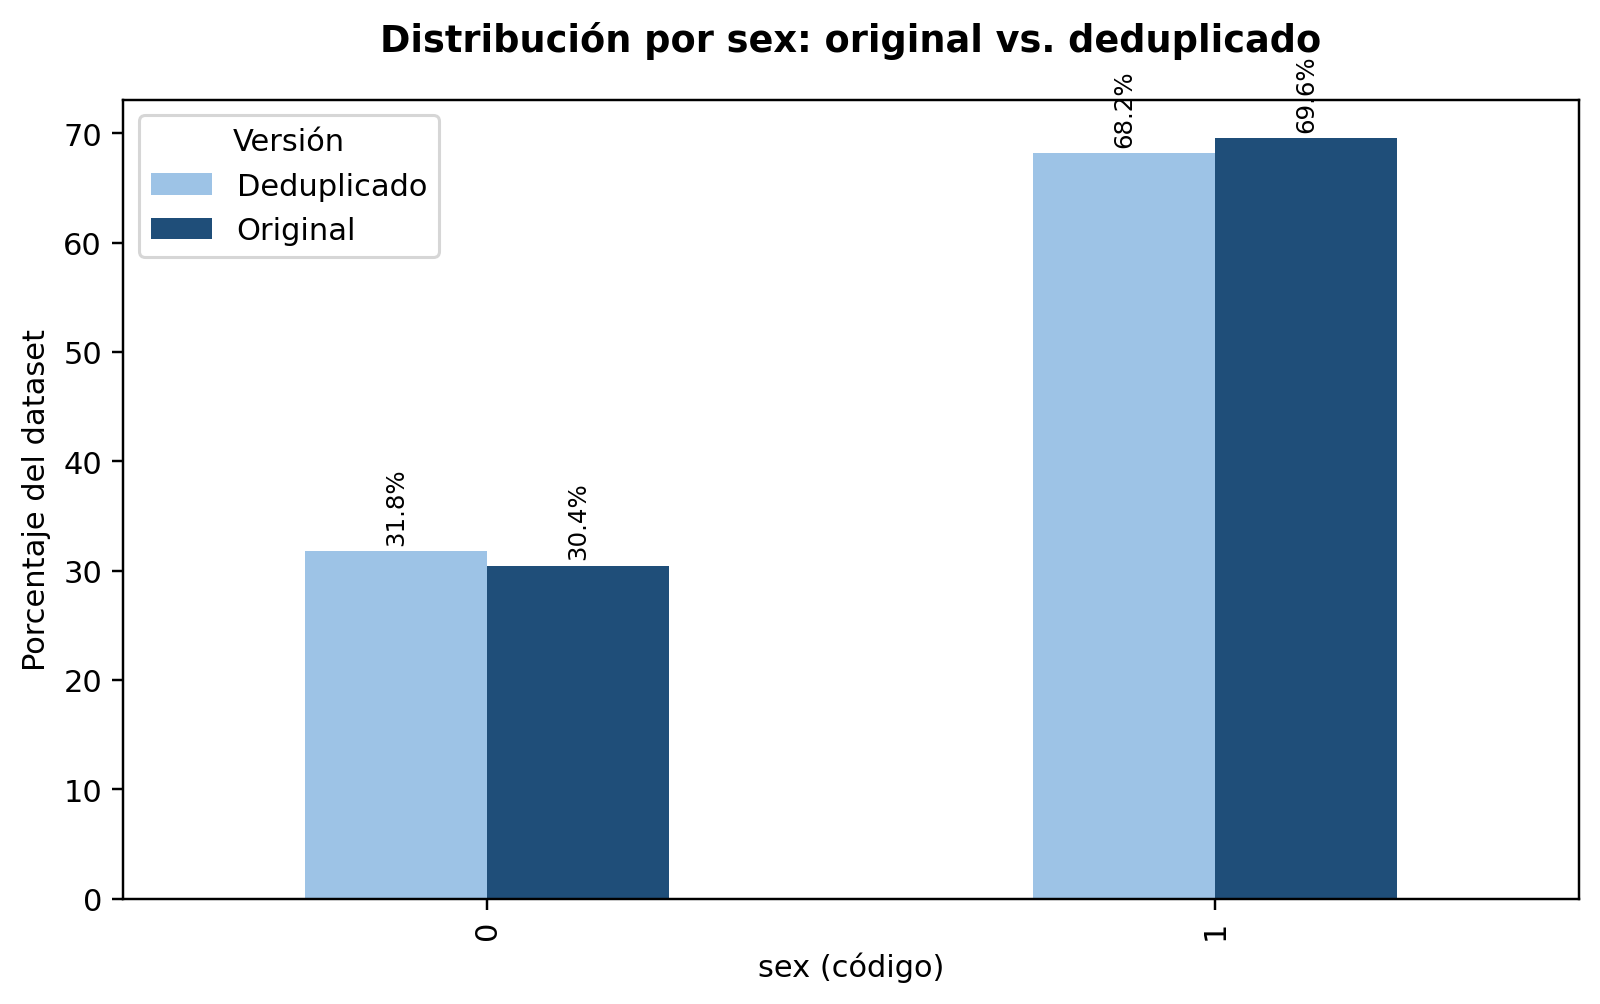
\includegraphics[width=0.82\textwidth]{../outputs/figures/comparacion_original_vs_unicos_sex.png}
  \caption{Comparación de la distribución de \texttt{sex} en el dataset original y deduplicado.}
  \label{fig:comparacion-sex}
\end{figure}

\begin{table}[H]
  \centering
  \caption{Distribución por rangos etarios: original versus deduplicado}
  \label{tab:comparacion-edad}
  \begin{tabular}{lrrr}
    \toprule
    Rango etario & Original (\%) & Deduplicado (\%) & Diferencia (pp) \\
    \midrule
    $<40$ & 5,56 & 4,97 & -0,59 \\
    40--49 & 23,12 & 23,84 & +0,72 \\
    50--59 & 41,17 & 41,39 & +0,22 \\
    60--69 & 26,83 & 26,49 & -0,34 \\
    70+ & 3,32 & 3,31 & -0,01 \\
    \bottomrule
  \end{tabular}
\end{table}

\begin{figure}[H]
  \centering
  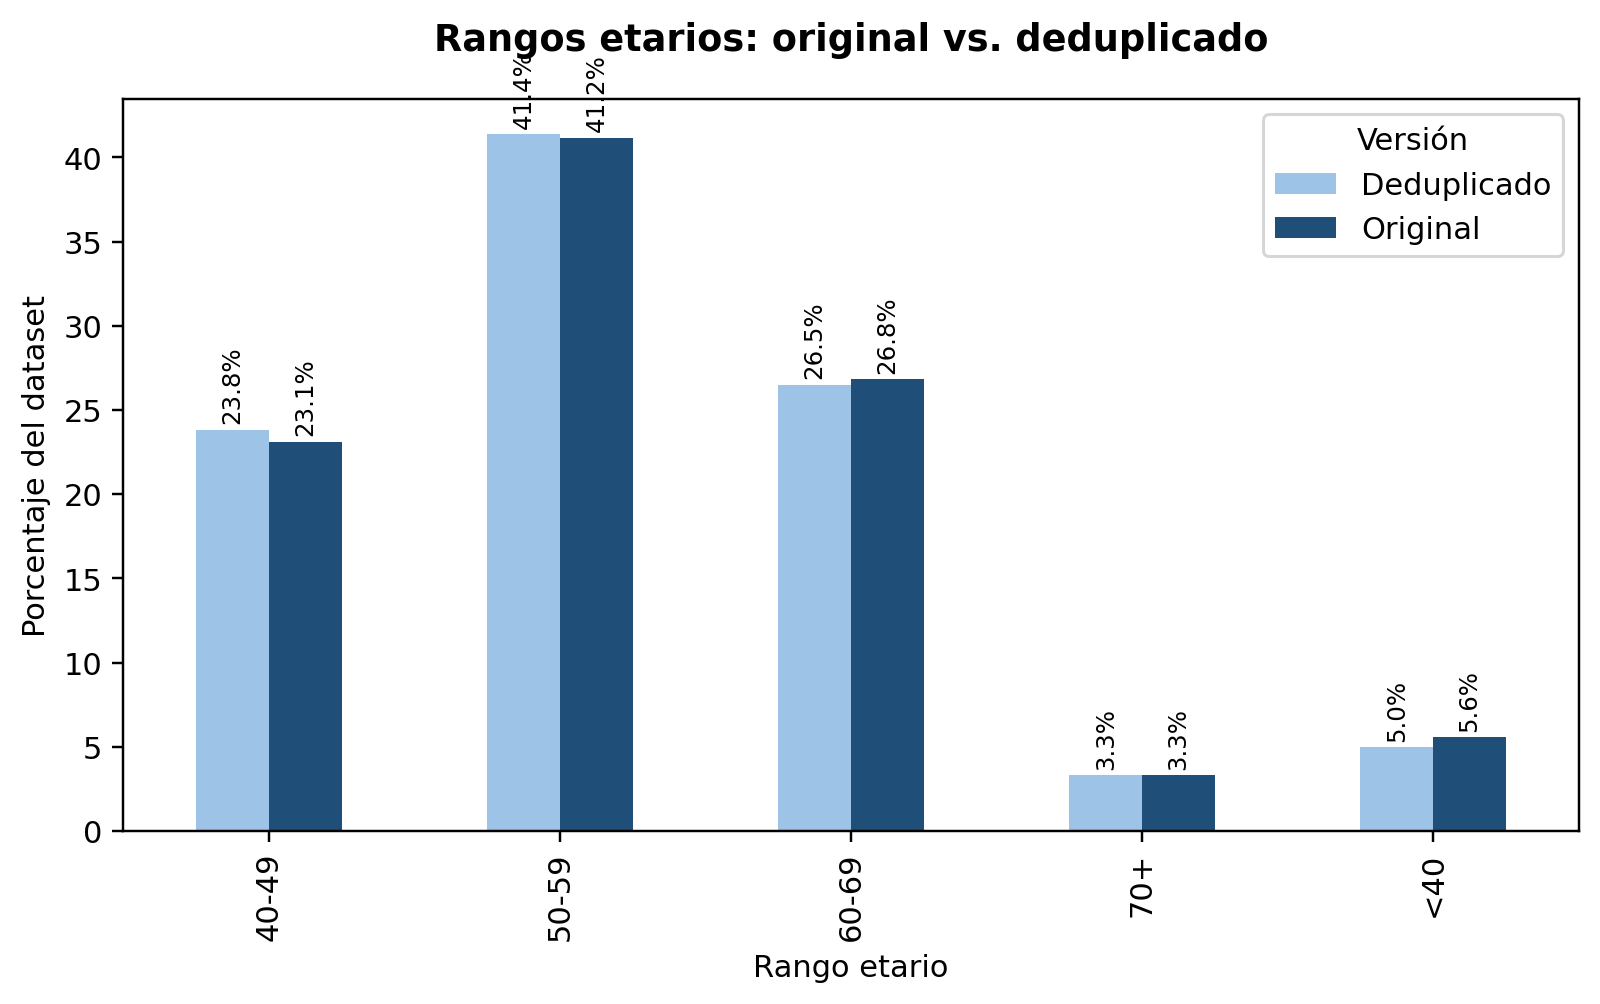
\includegraphics[width=0.82\textwidth]{../outputs/figures/comparacion_original_vs_unicos_edad.png}
  \caption{Comparación de los rangos etarios en el dataset original y deduplicado.}
  \label{fig:comparacion-edad}
\end{figure}

\subsection{Representación y subgrupos}

En la versión deduplicada, \texttt{sex}=0 concentra 96 registros (31,79\%) y \texttt{sex}=1 concentra 206 (68,21\%). Los rangos $<40$ (15 registros; 4,97\%) y 70+ (10; 3,31\%) disponen de menos evidencia que los rangos centrales. La \figref{fig:subgrupos-sex-edad} presenta los tamaños de las combinaciones \texttt{sex}$\times$rango etario. Los subgrupos \texttt{sex}=0 con $<40$ y con 70+ tienen cinco registros únicos cada uno; por ello, sus porcentajes de \texttt{target} son descriptivos y no constituyen evidencia de diferencias ni de sesgo demostrado.

\begin{figure}[H]
  \centering
  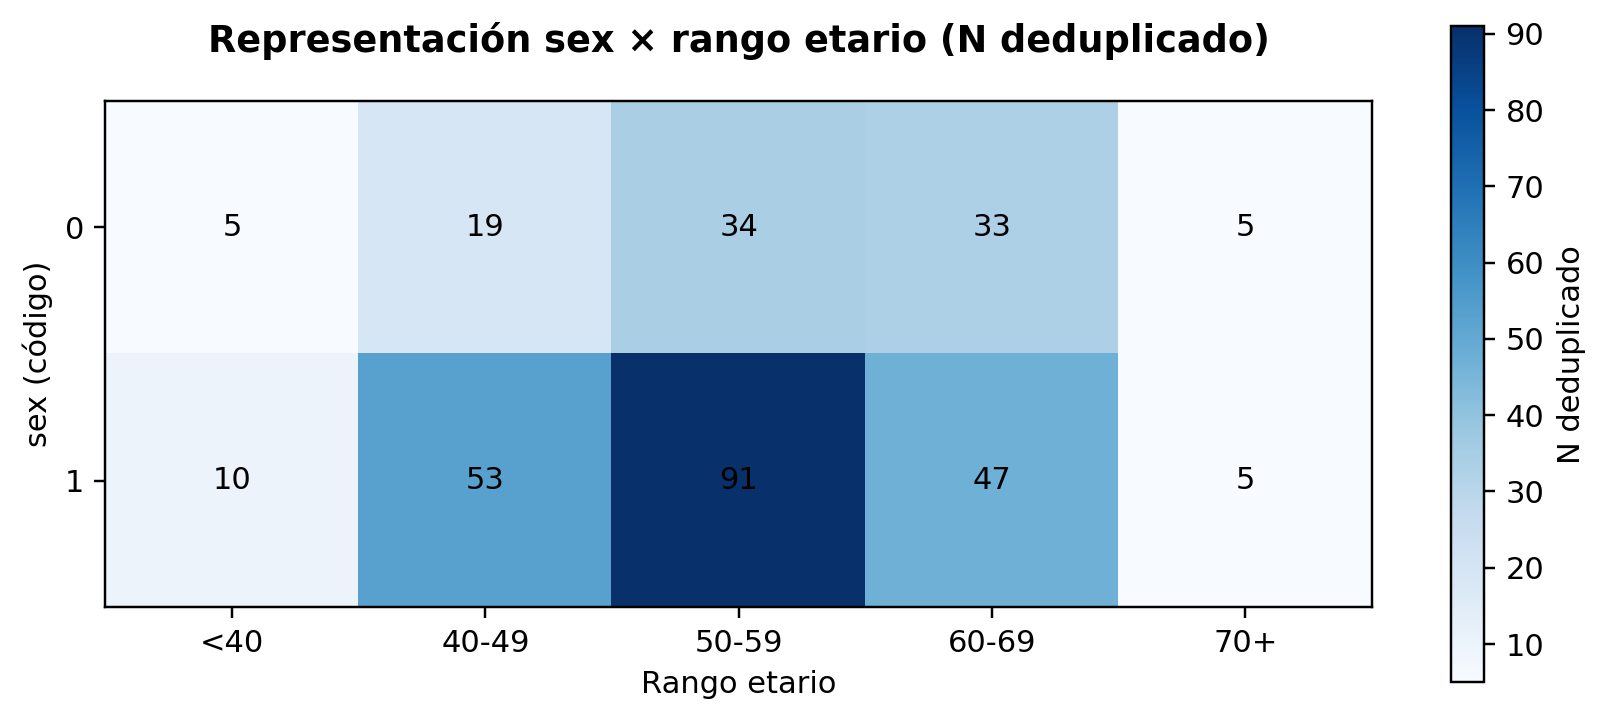
\includegraphics[width=0.88\textwidth]{../outputs/figures/representacion_sex_x_edad.png}
  \caption{Tamaño deduplicado de los subgrupos \texttt{sex}$\times$rango etario.}
  \label{fig:subgrupos-sex-edad}
\end{figure}

La evidencia sugiere posibles limitaciones de cobertura y generalización que deben validarse frente a la población objetivo. No permite afirmar discriminación, ni interpretar los códigos de \texttt{sex} sin confirmar su definición en la fuente oficial.

\section{Análisis D1}

\subsection{Alcance funcional}

La solución incluye: ingesta controlada de datasets cardiovasculares; validación de calidad; preparación para análisis y modelamiento; análisis exploratorio orientado al problema; comparación conceptual de modelos candidatos; métricas técnicas, estabilidad y evaluación por subgrupos; explicabilidad; una interfaz interna de referencia; versionado y trazabilidad del modelo; monitoreo de degradación, drift y fallos operacionales; y documentación de arquitectura, supuestos, riesgos, procedimientos y operación.

\subsection{Fuera de alcance}

Quedan expresamente fuera de alcance el diagnóstico médico automático, las recomendaciones automáticas de tratamiento, la negación o asignación automática de atención, la sustitución de personal sanitario, la integración productiva completa con HIS/EHR, el despliegue clínico definitivo y una plataforma nacional o multihospital desde el inicio. Estas exclusiones reducen el riesgo clínico y ético, respetan la información disponible y mantienen el proyecto dentro de un piloto institucional controlado.

\subsection{Arquitectura lógica común}

Para comparar las tres alternativas de manera justa, todas resuelven el mismo problema y mantienen el mismo alcance funcional. La cadena lógica es: fuente de datos hospitalaria, validación y control de calidad, almacenamiento estructurado o analítico, preparación y procesamiento, modelo o servicio de inferencia, API de aplicación, interfaz de usuario, y monitoreo, trazabilidad y respaldo.

Las diferencias de costo no deben provenir de comparar productos con funcionalidades distintas. Cambia dónde se ejecutan los componentes, quién los administra y cómo se distribuyen los costos y riesgos.

\section{Análisis D2}

\subsection{Alternativa Cloud}

La alternativa Cloud utiliza Google Cloud Platform (GCP) como proveedor de referencia. Esta elección no implica que GCP sea un ganador universal frente a AWS o Azure: la pauta exige evaluar infraestructura, almacenamiento, cómputo, redes, costos, escalabilidad y riesgos. GCP se selecciona para contar con un escenario reproducible, por su región en Santiago (\texttt{southamerica-west1}), la posibilidad de restringir ubicaciones de recursos, y la simplicidad de una arquitectura gestionada y portable \parencite{gcp-location,gcp-cloudrun}.

La aplicación se ejecuta en Cloud Run mediante contenedores Docker; Cloud SQL for PostgreSQL mantiene la persistencia estructurada; Cloud Storage almacena datasets, respaldos y artefactos; IAM, Secret Manager y Cloud Logging/Monitoring administran permisos, secretos y observabilidad. Python, Scikit-learn y SHAP conservan un stack portable y evitan una dependencia obligatoria de servicios propietarios de ML.

\subsection{Decisión sobre Vertex AI}

Vertex AI queda como capacidad futura y no como componente obligatorio del piloto. Una plataforma gestionada no sustituye la definición del problema, la validación de datos, la evaluación de sesgos, las métricas ni la operación. Su incorporación se evaluará si aumentan el volumen de datos, la cantidad de modelos, la frecuencia de reentrenamiento, la necesidad de pipelines administrados o el número de equipos trabajando sobre modelos.

\subsection{Beneficios, riesgos y componentes costables}

Los beneficios principales son elasticidad y pago por uso, menor inversión física inicial, servicios gestionados, escalamiento sin compra de hardware y una ruta de evolución hacia MLOps. Los trade-offs son dependencia de proveedor y conectividad, costos variables si no se controla el consumo, exposición por configuraciones IAM incorrectas, lock-in parcial y la necesidad de gobierno de datos y revisión legal.

Para la evaluación financiera deben considerarse la configuración inicial de GCP, seguridad y despliegue; Cloud Run; Cloud SQL; Cloud Storage y respaldos; red o egress cuando corresponda; monitoreo y logging; Secret Manager e IAM si tienen costo aplicable; RRHH de operación y seguridad; y seis ventanas de evaluación o reentrenamiento durante los 36 meses.

\section{Análisis D3}

\subsection{Alternativa Local u on-premise}

En la alternativa Local, los datos, el almacenamiento, el procesamiento, la inferencia y la aplicación permanecen dentro de la infraestructura hospitalaria. Los usuarios acceden por la red institucional a una aplicación interna, compuesta por Streamlit, FastAPI y Docker; PostgreSQL local persiste los datos; y el almacenamiento institucional mantiene los respaldos. El modelo utiliza Scikit-learn y SHAP, sin requerir GPU en la fase inicial.

El dimensionamiento exacto queda para costeo, pero se requiere un servidor físico o virtualizado con CPU multinúcleo, memoria y SSD suficientes; almacenamiento de respaldo segregado; segmentación de red; RBAC; MFA para administración; cifrado; EDR o antimalware; parcheo; logs y monitoreo; UPS; y un procedimiento probado de recuperación.

\subsection{Seguridad y continuidad}

Local no equivale a seguro por definición. Una infraestructura local mal mantenida puede exponerse a ransomware, credenciales comprometidas, software legado, ausencia de segmentación o respaldos inutilizables. El control directo de los datos implica transferir gran parte de la responsabilidad operacional al hospital. El contexto de ciberseguridad sectorial debe evaluarse conforme a los lineamientos del MINSAL \parencite{minsal-security,minsal-cyberplan}.

Sus beneficios son el control directo de datos e infraestructura, menor dependencia de Internet para uso interno e integración natural con la red institucional. Sus riesgos son mayor CAPEX, mantenimiento y parcheo a cargo de TI, costos de electricidad y respaldo, escalamiento menos elástico y una postura de ciberseguridad deficiente que puede anular la ventaja de control.

La evaluación financiera debe incorporar servidor o virtualización, almacenamiento y medios de respaldo, UPS y red cuando corresponda, implementación y hardening, electricidad, mantenimiento, repuestos o renovación, seguridad y licencias si la institución no las posee, RRHH TI y seguridad, pruebas de recuperación y las seis ventanas de evaluación o reentrenamiento.

\section{Análisis D4}

\subsection{Alternativa Híbrida}

La alternativa Híbrida conserva localmente la identidad, el registro maestro y la interfaz clínica; GCP concentra la capacidad analítica, el entrenamiento y la inferencia. Antes de transferir información, se aplican validación, minimización y pseudonimización. El resultado retorna a la aplicación clínica local y es utilizado por el profesional de salud.

La minimización restringe la transferencia a las variables necesarias para el propósito analítico. La pseudonimización mantiene el vínculo con la identidad real dentro del hospital. La solución además requiere TLS en tránsito, cifrado en reposo, IAM de mínimo privilegio, MFA, Secret Manager, auditoría en ambos ambientes y segregación de funciones. Pseudonimizar no convierte automáticamente la información clínica en datos no sensibles; se mantienen controles reforzados.

La inferencia se ejecuta en GCP para diferenciar la alternativa de la modalidad Local y reducir la infraestructura ML que debe operar el hospital. Si GCP o la conectividad no están disponibles, la atención clínica debe continuar sin el módulo predictivo, porque la plataforma es de apoyo y no es crítica.

\subsection{Distribución explícita de responsabilidades}

\begin{description}[style=nextline]
  \item[Permanece local] Identificadores directos del paciente, vínculo con la identidad, registro maestro clínico, aplicación o interfaz clínica interna, controles de acceso e integración interna.
  \item[Se ejecuta en GCP] Dataset analítico minimizado o pseudonimizado cuando corresponda, procesamiento y entrenamiento seleccionados, servicio de inferencia en Cloud Run, almacenamiento de artefactos y observabilidad cloud.
\end{description}

Los beneficios son el equilibrio entre control de identidad y elasticidad analítica, menor necesidad de comprar capacidad ML local anticipadamente, escalamiento gradual y una ruta futura hacia MLOps gestionado. Los trade-offs incluyen integración y operación dual, dependencia de conectividad para inferencia, riesgos de sincronización y transferencia, y costos operacionales distribuidos entre ambos entornos.

El costeo debe incluir infraestructura local mínima para registro maestro, interfaz e integración; configuración y seguridad de GCP; Cloud Storage y Cloud Run; cómputo temporal de entrenamiento; conectividad; monitoreo y respaldos en ambos ambientes; RRHH de integración, seguridad y operación; y seis ventanas de evaluación o reentrenamiento.

\section{Análisis D5}

\subsection{Herramientas y stack tecnológico}

La tecnología se define para evaluar factibilidad, costos, recursos y riesgos; el proyecto no exige construir todos los componentes. Se evita sobrearquitectura y se prioriza la portabilidad.

\subsection{Stack base común}

\begin{description}[style=nextline]
  \item[Python] Lenguaje principal por su ecosistema amplio de ciencia de datos, su carácter open source y su portabilidad.
  \item[Pandas y NumPy] Preparación y transformación de datos tabulares.
  \item[Scikit-learn] Modelamiento tradicional de clasificación tabular, sin sobredimensionar la plataforma ML.
  \item[PostgreSQL] Persistencia estructurada open source, disponible localmente o como servicio gestionado en GCP.
  \item[SHAP] Explicabilidad y análisis de influencia de variables.
  \item[FastAPI] Capa de servicio que desacopla el modelo de la interfaz.
  \item[Streamlit] Interfaz y dashboard de referencia para un prototipo interno sin licencias comerciales obligatorias.
  \item[Docker] Empaquetado consistente entre las tres alternativas.
  \item[Git] Versionado y trazabilidad de código, configuración y documentación.
\end{description}

Las tecnologías necesarias son Python, Pandas, Scikit-learn y PostgreSQL. Como capacidades operacionales se incorporan SHAP, FastAPI, Streamlit, Docker y Git cuando el proyecto se materializa como aplicación mantenible. MLflow, Vertex AI, orquestación u otros servicios avanzados quedan para una etapa de mayor volumen, más modelos, reentrenamiento frecuente o complejidad operacional.

Para GCP se consideran como servicios mínimos Cloud Run, Cloud SQL for PostgreSQL, Cloud Storage, IAM, Secret Manager y Cloud Logging/Monitoring. No se incorpora inicialmente Vertex AI, BigQuery, GKE/Kubernetes, Dataflow, Dataproc, GPU dedicada ni Cloud Healthcare API.

\section{Análisis D6}

\subsection{Justificación del enfoque adaptativo}

Un enfoque predictivo presupone requisitos tempranamente estables, menor incertidumbre, cambios controlados y retroalimentación más tardía. En este caso, los requisitos pueden evolucionar, existe incertidumbre en los datos, riesgos y solución, y se requieren experimentación y revisión continua. Por ello, la adecuación del enfoque predictivo es media y la del enfoque adaptativo es alta.

El enfoque adaptativo no significa improvisación. Conserva una línea base de alcance y objetivos, pero permite ciclos incrementales con entregables, responsables, revisiones y puntos de decisión. Esta modalidad permite ajustar la planificación frente a la evidencia de calidad de datos, desempeño, riesgos, privacidad, sesgos y factibilidad de las alternativas.

\subsection{Criterios completos de comparación}

\begin{description}[style=nextline]
  \item[Requisitos] En un enfoque predictivo son estables tempranamente; en uno adaptativo pueden evolucionar. En este caso, pueden evolucionar.
  \item[Incertidumbre] Es baja en el enfoque predictivo y media o alta en el adaptativo. El caso presenta incertidumbre alta en datos, riesgos y solución.
  \item[Cambios] El enfoque predictivo los minimiza o controla; el adaptativo los incorpora de forma planificada. En este proyecto son probables.
  \item[Retroalimentación] Es más tardía en el enfoque predictivo y frecuente en el adaptativo. El caso necesita retroalimentación frecuente.
  \item[Datos y modelos] El enfoque predictivo requiere mayor previsibilidad; el adaptativo permite experimentar. El caso presenta incertidumbre en esta materia.
  \item[Riesgos] En el enfoque predictivo se planifican principalmente al inicio; en el adaptativo se revisan durante los ciclos. El caso requiere revisión continua.
  \item[Adecuación] La adecuación predictiva es media y la adaptativa es alta; por ello se selecciona el enfoque adaptativo.
\end{description}

El efecto transversal es claro: la EDT y la carta Gantt deben considerar revisiones y capacidad de ajuste; finanzas debe presupuestar iteración y contingencia; riesgos debe actualizarse al aparecer nueva evidencia; y la evaluación ética debe acompañar el ciclo completo.

\section{Evaluación financiera Cloud, Local e Híbrida (D7--D11)}

Esta sección incorpora la evaluación financiera preparada por Ignacio Silva para el piloto institucional de apoyo a la prevención cardiovascular. Se comparan las alternativas Cloud, Local e Híbrida bajo las mismas condiciones operacionales durante 36 meses. Los montos están expresados en pesos chilenos (CLP), incluyen una contingencia de 10\% y corresponden a estimaciones de planificación, no a cotizaciones vinculantes \parencite{ignacio-financiero}.

\subsection{Modelo de costos y supuestos comunes (D7)}

Se utiliza el Costo Total de Propiedad (TCO) a 36 meses: CAPEX, implementación y RRHH, OPEX recurrente, mantención y contingencia. El horizonte permite comparar alternativas con inversión inicial y alternativas de pago mensual sin extender la proyección a un plazo excesivamente incierto. El \tabref{tab:fin-supuestos} resume los supuestos comunes que aseguran comparabilidad.

\begin{table}[H]
  \centering
  \caption{Supuestos financieros comunes para las tres alternativas}
  \label{tab:fin-supuestos}
  \small
  \begin{tabular}{ll}
    \toprule
    Supuesto & Valor utilizado \\
    \midrule
    Horizonte & 36 meses \\
    Escenario & Piloto institucional controlado \\
    Usuarios y concurrencia & A1: 20/5; A2: 25/6; A3: 30/8 \\
    Datos de planificación & 10.000 iniciales; 5.000 nuevos en A1; crecimiento 10\% anual \\
    Mantenimiento del modelo & Seis ventanas en 36 meses \\
    Continuidad & 99\% horario operacional; RTO 8 h; RPO 24 h \\
    Moneda y tipo de cambio & CLP; \$930 por USD \\
    Licencias base & \$0; stack open source \\
    Contingencia & 10\% del subtotal \\
    \bottomrule
  \end{tabular}
\end{table}

El modelo de RRHH considera 220 h de Data/ML, 120 h de Desarrollo/Data Engineering y 72 h de Seguridad y Gobierno. La operación específica agrega 120 h de Cloud/DevOps, 300 h de SysAdmin Local o 280 h de Integración/DevOps Híbrida. En consecuencia, los totales son 532 h para Cloud, 712 h para Local y 692 h para Híbrida. Las tarifas y horas son supuestos de planificación y cualquier variación debe recalcular el TCO.

\subsection{Alternativa Cloud (D8)}

Cloud utiliza GCP en la región de Santiago, con Cloud Run, Cloud SQL para PostgreSQL, Cloud Storage, respaldo, monitoreo y gestión de secretos. Se excluyen Vertex AI, BigQuery, GKE, Dataflow, Dataproc y GPU dedicada porque el volumen y la frecuencia de reentrenamiento del piloto no los justifican. La fórmula de reproducción de las partidas GCP es: USD/mes $\times$ 36 meses $\times$ \$930 CLP/USD. Los consumos son bolsas de planificación y deben contrastarse con una exportación fechada de Google Cloud Pricing Calculator antes de contratar.

\begin{table}[H]
  \centering
  \caption{TCO Cloud a 36 meses}
  \label{tab:tco-cloud}
  \small
  \begin{tabular}{lr}
    \toprule
    Partida & CLP \\
    \midrule
    Cloud SQL & \$768.024 \\
    Cloud Run & \$96.720 \\
    Storage y respaldo & \$111.600 \\
    Logging, monitoreo, secretos y red & \$279.000 \\
    Cómputo temporal de reentrenamiento & \$55.800 \\
    IVA GCP & \$249.117 \\
    RRHH Cloud & \$8.272.000 \\
    \midrule
    Subtotal Cloud & \$9.832.261 \\
    Contingencia 10\% & \$983.226 \\
    \textbf{TCO Cloud 36 meses} & \textbf{\$10.815.487} \\
    \bottomrule
  \end{tabular}
\end{table}

El componente predominante es RRHH: \$8.272.000, equivalente al 76,5\% del TCO Cloud corregido. Por ello, una discusión centrada solamente en Cloud Run u hosting no representa el principal impulsor de costo.

\subsection{Alternativas Local e Híbrida (D9--D10)}

Local conserva aplicación, procesamiento y PostgreSQL dentro del hospital. Aporta control directo del entorno, pero transfiere al hospital la responsabilidad de parches, respaldos, recuperación, monitoreo, energía y renovación de componentes. Híbrida conserva registro maestro, identidad, interfaz e integración en el hospital, mientras entrenamiento e inferencia se realizan en GCP con datos necesarios y pseudonimizados. Reduce infraestructura local, pero exige integración, seguridad y soporte en dos ambientes.

\begin{table}[H]
  \centering
  \caption{Resumen de TCO por alternativa a 36 meses}
  \label{tab:tco-comparacion}
  \small
  \begin{tabular}{lrrr}
    \toprule
    Alternativa & CAPEX estimado & RRHH & TCO 36 meses \\
    \midrule
    Cloud & Muy bajo & \$8.272.000 & \$10.815.487 \\
    Local & Alto & \$9.952.000 & \$16.893.013 \\
    Híbrida & Medio & \$10.832.000 & \$15.696.956 \\
    \bottomrule
  \end{tabular}
\end{table}

Los valores de hardware Local e Híbrido son referencias pendientes de respaldo documental: proveedor, URL o cotización, fecha, especificación comparable y precio con o sin IVA. Por ello se mantienen para comparación, pero deben actualizarse antes de una contratación. En Híbrida, el mayor esfuerzo de RRHH responde a sincronización, seguridad y soporte de dos entornos.

\subsection{Costo-beneficio, sensibilidad y recomendación (D11)}

Cloud presenta el menor TCO: ahorra \$6.077.526 frente a Local (36,0\% del TCO Local) y \$4.881.469 frente a Híbrida (31,1\% del TCO Híbrido). Esta recomendación es exclusivamente financiera. Solo se mantiene si la evaluación ética, legal y de riesgos autoriza el tratamiento de datos sensibles en GCP Chile bajo las medidas definidas; si no se satisface esa condición, Híbrida se mantiene como alternativa de respaldo para evaluación integral.

\begin{table}[H]
  \centering
  \caption{Escenarios de sensibilidad financiera}
  \label{tab:sensibilidad-financiera}
  \small
  \begin{tabular}{lrrr}
    \toprule
    Escenario & Cloud & Local & Híbrida \\
    \midrule
    Tipo de cambio +15\% & +\$234 mil & Sin efecto relevante & +\$162 mil \\
    Cuatro reentrenamientos/año & +\$434 mil & +\$384 mil & +\$530 mil \\
    Usuarios 50\% sobre el plan & +\$291 mil & +\$180 mil & +\$350 mil \\
    Falla de hardware local & Sin efecto directo & +\$1,2 a \$2,0 millones & +\$500 a \$900 mil \\
    \bottomrule
  \end{tabular}
\end{table}

Los riesgos financieros a integrar en la matriz de riesgos son variación USD/CLP y consumo cloud, servicios no previstos, falla o renovación de hardware, subestimación de horas, tratamiento tributario distinto e integración más compleja en Híbrida. Las medidas propuestas incluyen contingencia, alertas y límites de gasto, etiquetado por servicio, inventario y garantía de hardware, control de horas en la Gantt y validación tributaria previa a contratación.

\section{Planificación integrada, Gantt y recursos (D12--D14)}

Esta sección incorpora la planificación integrada elaborada por Fabián Leal. Traduce la línea base técnica D1--D6 y el TCO D7--D11 en un plan ejecutable y trazable \parencite{fabian-planificacion}. Usa Cloud/GCP como escenario base de planificación porque es la alternativa financieramente preferida; esto no constituye la recomendación integral definitiva, que continúa condicionada a riesgos, ética, legalidad y validación local. Distingue dos horizontes: un piloto de implementación de 10 semanas y una operación financiera y de gobierno de 36 meses. El piloto de 10 semanas es un supuesto de planificación; el horizonte de 36 meses incluye ingesta batch diaria, RTO de 8 h, RPO de 24 h y seis ventanas semestrales de evaluación y eventual reentrenamiento.

\subsection{Estructura de Desglose del Trabajo (D12)}

La EDT se organiza en seis paquetes de trabajo: (1) gobierno, alcance y línea base; (2) dataset gobernado y pipeline batch; (3) modelos candidatos, explicabilidad y servicio de inferencia; (4) validación técnica, ética y de sesgos; (5) plataforma Cloud segura y piloto; y (6) continuidad operacional y seis ventanas de evaluación. Los entregables de segundo nivel incluyen alcance aprobado, recursos y control TCO, dataset pseudonimizado, almacenamiento seguro, modelos y explicabilidad, auditoría por subgrupos, protocolo Human in the Loop, monitoreo de deriva, entorno GCP, continuidad y reportes semestrales.

\subsection{Carta Gantt del piloto (D13)}

El \tabref{tab:gantt-piloto} muestra la planificación de 10 semanas. Los solapamientos corresponden a actividades preparatorias compatibles con un enfoque adaptativo; ningún entregable atraviesa su punto de control sin evidencia del predecesor.

\begin{table}[H]
  \centering
  \caption{Carta Gantt resumida del piloto de 10 semanas}
  \label{tab:gantt-piloto}
  \scriptsize
  \resizebox{\textwidth}{!}{%
  \begin{tabular}{llcccccccccc}
    \toprule
    EDT & Entregable & S1 & S2 & S3 & S4 & S5 & S6 & S7 & S8 & S9 & S10 \\
    \midrule
    1.1 & Alcance y requerimientos aprobados & $\bullet$ & $\bullet$ & & & & & & & & \\
    1.2--1.4 & Recursos y control TCO & & $\bullet$ & $\bullet$ & $\bullet$ & $\bullet$ & $\bullet$ & $\bullet$ & $\bullet$ & $\bullet$ & $\bullet$ \\
    2.1--2.3 & Dataset inicial, gobierno e ingesta batch & & $\bullet$ & $\bullet$ & $\bullet$ & & & & & & \\
    2.4--2.5 & Dataset analítico y almacenamiento seguro & & & $\bullet$ & $\bullet$ & & & & & & \\
    3.1--3.2 & Modelos candidatos y explicabilidad & & & & $\bullet$ & $\bullet$ & & & & & \\
    3.3--3.4 & Servicio de inferencia y pruebas & & & & & $\bullet$ & $\bullet$ & & & & \\
    4.1--4.2 & Validación técnica y por subgrupos & & & & & $\bullet$ & $\bullet$ & & & & \\
    4.3--4.4 & Human in the Loop y deriva & & & & & & $\bullet$ & & & & \\
    5.1--5.2 & Cloud, IAM y secretos & & & & & & $\bullet$ & $\bullet$ & & & \\
    5.3--5.4 & Observabilidad, costos, backups y RTO/RPO & & & & & & & $\bullet$ & $\bullet$ & & \\
    5.5 & Piloto controlado & & & & & & & & $\bullet$ & & \\
    1.5 & Cierre del piloto & & & & & & & & & $\bullet$ & $\bullet$ \\
    \bottomrule
  \end{tabular}}
\end{table}

La ruta crítica es: alcance aprobado $\rightarrow$ dataset analítico $\rightarrow$ modelo candidato $\rightarrow$ servicio de inferencia $\rightarrow$ validación técnica y por subgrupos $\rightarrow$ gate Human in the Loop $\rightarrow$ piloto $\rightarrow$ cierre.

\subsection{Hitos, dependencias y continuidad (D14)}

Los hitos H1 a H6 ocurren en las semanas 2, 4, 5, 6, 8 y 10, respectivamente: aprobación de alcance y TCO; dataset limpio y pseudonimizado; baseline y explicabilidad; certificación ética, SLA y continuidad; puesta en marcha; y cierre del piloto. H7 se repite en los meses 6, 12, 18, 24, 30 y 36. En cada H7 se evalúan deriva, desempeño, equidad y explicabilidad; un nuevo modelo solo se publica con validación y aprobación clínica.

\begin{table}[H]
  \centering
  \caption{Asignación de recursos de RRHH para la alternativa Cloud}
  \label{tab:rrhh-cloud}
  \small
  \begin{tabular}{lrrr}
    \toprule
    Rol & Implementación & Mantención & Total \\
    \midrule
    Data Scientist & 100 h & 120 h & 220 h \\
    Desarrollo / Data Engineering & 80 h & 40 h & 120 h \\
    Seguridad y Gobierno & 32 h & 40 h & 72 h \\
    DevOps / Cloud Ops & 60 h & 60 h & 120 h \\
    \midrule
    \textbf{Total Cloud} & \textbf{272 h} & \textbf{260 h} & \textbf{532 h} \\
    \bottomrule
  \end{tabular}
\end{table}

Las dependencias principales son de fin a inicio: los modelos requieren el dataset analítico; el servicio requiere un modelo candidato; la validación requiere resultados y pruebas; el piloto exige el gate ético, seguridad, observabilidad y continuidad; y el cierre depende del piloto. Los riesgos de planificación entregados para consolidación incluyen desviación de horas de RRHH, retraso ético/legal, fallas de ingesta batch y volatilidad cambiaria.

Los criterios de aceptación establecen: comparación del modelo candidato con el baseline usando criterios acordados con la contraparte clínica; explicabilidad y supervisión humana; RTO $\leq$ 8 h y RPO $\leq$ 24 h verificados mediante restauración; pseudonimización, Secret Manager e IAM de mínimo privilegio; y control contra TCO Cloud de \$10.815.487, 532 h de RRHH y contingencia de \$983.226.

\section{Discusión}\label{sec:discusion}

\subsection{Supuestos comunes para las tres alternativas}

Las tres alternativas se evalúan durante 36 meses. El horizonte permite comparar CAPEX y OPEX sin castigar artificialmente la inversión inicial de la alternativa Local ni proyectar precios y tecnología a un plazo excesivamente incierto. El TCO debe incluir costos iniciales, implementación, OPEX recurrente, costos periódicos, RRHH y contingencia, respetando la periodicidad de cada partida y evitando doble conteo.

La etapa evaluada es un piloto institucional funcional y mantenible. Incluye infraestructura, aplicación, datos, seguridad, respaldo, monitoreo, RRHH y operación; no incluye integración total con los sistemas del hospital, disponibilidad crítica 24/7 ni despliegue nacional. El cronograma de implementación es independiente del horizonte financiero.

Se consideran 20 usuarios autorizados y hasta 5 concurrentes en el año 1; 25 y 6 en el año 2; y 30 y 8 en el año 3. La curva representa adopción gradual del área cardiovascular y preventiva, no crecimiento de la dotación hospitalaria. Se asume una carga histórica de 10.000 registros, 5.000 nuevos o actualizados durante el primer año, crecimiento de 10\% anual y un acumulado aproximado de 15.000, 20.500 y 26.550 registros en los años 1, 2 y 3. Para sensibilidad se proponen escenarios de 2.500, 5.000 y 10.000 registros anuales iniciales. La referencia de demanda de cardiología en hospitales públicos de Santiago se utiliza solo como orden de magnitud, no como dato del hospital ficticio \parencite{lagos2024,sotero-about,sotero-cardiology}.

La continuidad común exige disponibilidad objetivo de 99\% en horario operacional, RTO máximo de 8 horas, RPO máximo de 24 horas, backup operativo diario, backup completo semanal, retención mínima de 30 días y prueba mensual de restauración. La atención debe continuar si la plataforma no está disponible.

\subsection{Detalle de supuestos y sensibilidad}

La estimación de 20 usuarios autorizados se distribuye aproximadamente entre 15 profesionales del proceso cardiovascular o preventivo, 3 personas de coordinación o gestión y 2 perfiles técnicos. Es un supuesto de dimensionamiento, no una estadística del hospital ficticio. La referencia histórica de una unidad de cardiología infantil con 14 integrantes y el dato institucional de más de 5.000 funcionarios se usan solo para contextualizar el orden de magnitud \parencite{sotero-about,sotero-cardiology}.

El escenario de volumen utiliza 10.000 registros históricos al inicio; 5.000 registros nuevos o actualizados en el año 1; 5.500 en el año 2; y 6.050 en el año 3. Los acumulados estimados son 10.000 al inicio, 15.000, 20.500 y 26.550 respectivamente. Los escenarios de sensibilidad son bajo, con 2.500 registros anuales iniciales; base, con 5.000; y alto, con 10.000.

Para la sensibilidad financiera también puede analizarse un escenario de cuatro ciclos de reentrenamiento por año, frente a los dos ciclos semestrales de la línea base. Las alternativas deben costearse para el mismo nivel de continuidad; ninguna puede parecer más barata por ofrecer menor respaldo o recuperación.

\subsection{Comparación consolidada}

\begin{description}[style=nextline]
  \item[Cloud GCP] Los datos, entrenamiento e inferencia se ejecutan en GCP y Cloud Run; la interfaz es cloud autenticada. Tiene CAPEX bajo, OPEX variable y RRHH, escalabilidad alta y rápida, alta dependencia de Internet, menor control físico y complejidad media. El MLOps avanzado queda para una etapa futura si se justifica.
  \item[Local] Los datos, entrenamiento e inferencia permanecen en el hospital y la interfaz opera en la red interna. Tiene CAPEX mayor y costos de operación y mantenimiento local, escalabilidad posible pero menos elástica, baja dependencia de Internet, mayor control físico y complejidad media. El MLOps avanzado es posible, con mayor esfuerzo local.
  \item[Híbrida] La identidad, el registro maestro y la interfaz permanecen locales; el dataset analítico controlado, el entrenamiento y la inferencia se ejecutan en GCP. Tiene CAPEX intermedio, operación dual, costos cloud y RRHH, alta escalabilidad analítica, dependencia media o alta de Internet para inferencia, mayor control de identidad y complejidad alta. El MLOps avanzado queda para cloud si se justifica.
\end{description}

\subsection{Riesgos y elementos pendientes}

Los riesgos transversales incluyen calidad de datos, duplicados, cambios de esquema, retrasos, fallos de pipeline, drift, degradación del modelo, baja explicabilidad y fallos de respaldo. Cloud agrega dependencia de GCP, conectividad, costos variables, errores IAM, exposición y lock-in; Local incorpora ransomware, software desactualizado, fallos de servidor o UPS, respaldo comprometido, falta de personal especializado y segmentación deficiente; Híbrida añade fallos de sincronización, inconsistencias, exposición durante transferencia y doble operación.

No se cierran aún el precio y sizing final de GCP, el hardware local exacto, las horas por rol y duración de implementación, la alternativa financiera preferida, la matriz de riesgos residual, el análisis legal vigente, los sesgos e impactos éticos finales ni la alternativa recomendada. Estas decisiones requieren la integración de los responsables correspondientes.

La auditoría de aceptación concluye que las alternativas comparten problema y alcance, las herramientas tienen función justificada y la metodología está argumentada. Finanzas y planificación pueden trabajar con los supuestos y handoffs definidos, aunque los precios, dimensionamientos y análisis integrales quedan pendientes.

\section{Conclusiones}

La línea base conceptual D1 a D6 define una plataforma de apoyo a la prevención cardiovascular, no un sistema de diagnóstico autónomo. La comparación entre Cloud, Local e Híbrida es válida porque las tres alternativas conservan el mismo alcance, los mismos supuestos de usuarios, registros, operación, reentrenamiento y continuidad.

El stack propuesto es portable, mantenible y predominantemente open source. GCP se usa como escenario Cloud concreto, sin imponer servicios avanzados de ML antes de que su necesidad esté demostrada. La alternativa Local ofrece control directo, pero exige una operación y postura de seguridad sostenida. La alternativa Híbrida equilibra control de identidad local con elasticidad analítica en cloud, a costa de mayor integración y operación dual.

El enfoque adaptativo es consistente con la incertidumbre de los datos y del proyecto. El informe maestro declara el proyecto \textbf{viable condicionado} y selecciona Cloud/GCP como alternativa integral recomendada para el piloto, con TCO oficial de \$10.815.487 CLP a 36 meses. La selección está condicionada al cumplimiento verificable de CA-E01 a CA-E10, autorización y gobierno de datos aplicables, controles técnicos y de seguridad, aceptación de riesgos y validación local; no declara cumplimiento legal definitivo ni umbrales clínicos no acordados. Híbrida se mantiene como contingencia ante una no aprobación legal, institucional o de gobierno de datos de Cloud. Local es técnicamente viable, pero no se recomienda para este piloto por su mayor TCO y carga operacional.

\section{Recomendaciones}

\subsection{Handoff para evaluación financiera}

La evaluación financiera debe costear Cloud, Local e Híbrida con los mismos supuestos de horizonte, piloto, usuarios, volumen, actualización, mantenimiento de modelo y continuidad. Cloud debe considerar configuración, seguridad, despliegue, Cloud Run, Cloud SQL, Storage, red, monitoreo, soporte, RRHH y cómputo temporal; no debe suponer entrenamiento 24/7 ni Vertex AI obligatorio. Local debe incluir CAPEX de infraestructura, hardening, electricidad, mantenimiento, seguridad, backup, soporte y RRHH, dimensionado al menos para el escenario del año 3. Híbrida debe sumar infraestructura local mínima, costos cloud e integración, conectividad, monitoreo de ambos ambientes y el esfuerzo de operación dual.

La sensibilidad mínima debe variar registros anuales (2.500 y 10.000 frente al escenario base de 5.000), reentrenamientos (4 frente a 2 por año), usuarios cuando corresponda y el componente dominante de costo de cada arquitectura.

\subsection{Fórmula y reglas de costeo}

La estructura común es \(\mathrm{TCO}_{36\,meses}=\) CAPEX o costos iniciales + implementación + suma de OPEX recurrente del horizonte + costos periódicos + RRHH + contingencia justificada. Cada partida debe respetar su periodicidad real para evitar multiplicaciones incorrectas o doble conteo.

Cloud debe dimensionarse para 20, 25 y 30 usuarios; 5, 6 y 8 usuarios concurrentes; 10.000 registros históricos más el crecimiento definido; batch diario; y los RTO/RPO comunes. Local debe soportar al menos el escenario del año 3 sin una sustitución completa por el crecimiento base. Híbrida debe incluir el costo y el impacto de seguridad y sincronización entre ambos ambientes.

\subsection{Handoff para planificación, riesgos e integración}

La EDT y carta Gantt deben orientarse a entregables: inicio y alcance, datos, preparación, análisis y modelo, validación técnica y ética, infraestructura o piloto, documentación y cierre. Deben incluir backup, monitoreo, recuperación y mantenimiento como trabajo gestionable, y separar la duración de implementación de los 36 meses financieros.

La matriz de riesgos debe consolidar los riesgos técnicos expuestos en la Sección~\ref{sec:discusion} con los riesgos financieros, éticos, legales y de planificación. Para la integración ética, debe mantenerse que el sistema no reemplaza al profesional, que el dataset actual es un prototipo y que Cloud e Híbrida tratan datos sensibles fuera del entorno local. La recomendación final no debe decidirse solo por precio.

\subsection{Handoffs nominales y matriz de riesgos semilla}

Ignacio recibe los componentes, supuestos y fórmulas para la evaluación financiera. El responsable de EDT o Carta Gantt recibe D1 como línea base de alcance, usuarios y límites, junto con la necesidad de una EDT orientada a entregables. Vicente recibe los riesgos técnicos preliminares para consolidarlos con riesgos financieros, éticos, legales y de planificación. César recibe las restricciones para la integración ética y la recomendación final.

\begin{description}[style=nextline]
  \item[Transversal] Calidad de datos, duplicados, cambios de esquema, datos retrasados, fallos del pipeline, drift, degradación del modelo, baja explicabilidad y fallo de backup.
  \item[Cloud] Dependencia de GCP, pérdida de conectividad, costos variables, error IAM, exposición de datos, indisponibilidad del proveedor y lock-in.
  \item[Local] Ransomware, software desactualizado, fallo de servidor o UPS, backup comprometido, falta de personal especializado, escalabilidad lenta y mala segmentación.
  \item[Híbrida] Fallo de sincronización, inconsistencia entre entornos, exposición durante transferencia, mayor complejidad, dependencia de Internet para inferencia y doble operación.
  \item[Continuidad] RTO superior a 8 horas, RPO superior a 24 horas, restauración fallida y pérdida de datos analíticos.
  \item[Mantenimiento ML] Reentrenar con datos defectuosos, nueva versión peor, incremento de sesgos, pérdida de trazabilidad o publicación sin aprobación.
\end{description}

\subsection{Matriz de trazabilidad de decisiones}

\begin{description}[style=nextline]
  \item[Apoyo preventivo] Se fundamenta en el caso y EA1; se usa para ética y para delimitar el alcance de planificación.
  \item[Tres alternativas con mismo alcance] Se fundamenta en el Plan Maestro; permite comparación financiera y análisis de riesgos equivalentes.
  \item[GCP como referencia Cloud] Se fundamenta en la decisión de diseño, región de Santiago y simplicidad; permite tarifar Cloud y revisar sus riesgos.
  \item[Stack portable y open source] Se fundamenta en costo-beneficio y comparabilidad; sirve para licencias y planificación de recursos.
  \item[Sin Vertex AI inicial] Evita sobrearquitectura a la escala actual; define el costo base y los gatillos de escalamiento futuro.
  \item[Local con seguridad reforzada] Se fundamenta en EA1 y contexto MINSAL; alimenta ciberseguridad, costos de seguridad y continuidad.
  \item[Híbrida con minimización y pseudonimización] Se fundamenta en privacidad y diseño del caso; alimenta ética, legalidad, riesgos e integración.
  \item[Metodología adaptativa] Se fundamenta en incertidumbre; define ciclos, hitos y revisiones de EDT o Gantt.
  \item[Horizonte de 36 meses] Hace comparables CAPEX y OPEX para el TCO.
  \item[Piloto controlado] Evita comparar un notebook trivial con una producción ficticia y delimita el alcance de todos los análisis.
  \item[Crecimiento de usuarios, volumen, batch y reentrenamiento] Entregan bases comunes para sizing, costos, operación, riesgos y validación.
  \item[99\%, RTO 8 h y RPO 24 h] Definen respaldo, pruebas, planificación y riesgos de continuidad.
\end{description}

\subsection{Auditoría de aceptación D1 a D6}

La línea base cumple con que las tres alternativas resuelven el mismo problema y alcance; cada herramienta tiene una función y motivo; y la metodología está argumentada, no solo nombrada. También permite a Ignacio costear sin inventar componentes mediante los supuestos y el handoff, aunque aún faltan precios y sizing exactos. Permite construir EDT y Gantt sin reinterpretar el alcance; distingue proyecto conceptual de ejecución real; mantiene fuentes y supuestos trazables; y prohíbe declarar una alternativa ganadora antes de integrar finanzas, riesgos y ética.

\subsection{Checklist de integración}

\begin{itemize}
  \item Mantener D1 a D6 como línea base y comunicar cualquier cambio a finanzas, planificación, riesgos e integración.
  \item No declarar una alternativa ganadora antes de terminar los análisis financiero, de riesgos y ético.
  \item Usar los mismos supuestos para Cloud, Local e Híbrida.
  \item Distinguir datos reales, referencias externas y supuestos de planificación.
  \item Respaldar cada cifra de costos con tarifario, cotización o supuesto reproducible.
  \item Conservar el carácter de apoyo preventivo y no diagnóstico autónomo.
  \item Sintetizar el informe final EP1 a 4--6 páginas, con letra 11, interlineado simple y estilo APA; este documento maestro puede ser más extenso.
  \item Corregir la consistencia del responsable de EDT o Gantt antes de la entrega final, si existen nombres distintos en los documentos del equipo.
\end{itemize}

\section{Referencias}
\nocite{*}
\printbibliography[heading=none]


\end{document}
